\documentclass[conference]{IEEEtran}
\IEEEoverridecommandlockouts

\usepackage[english]{babel}
\usepackage{cite}
\usepackage{amsmath,amssymb}
\usepackage{graphicx}
\usepackage{booktabs}
\usepackage{array}
\usepackage{multirow}
\usepackage[hidelinks]{hyperref}

\graphicspath{{figures/}}

\begin{document}

\title{PAM-VLM: Disagreement-Aware Audio--Visual Emotion Recognition
with Language-Model Reconciliation}

\author{
  \IEEEauthorblockN{Tuan-Anh Pham}
  \IEEEauthorblockA{
    \textit{Faculty of Electrical and Electronic Engineering}\\
    \textit{Phenikaa University}\\
    Hanoi, Vietnam\\
    \href{mailto:ptattmpxd01012004@gmail.com}{ptattmpxd01012004@gmail.com}
  }
}

\maketitle

\begin{abstract}
Audio--visual emotion recognition combines vocal and facial evidence, but
published CREMA-D results are difficult to compare because the dataset has no
official evaluation partition. This paper presents PAM-VLM, a multimodal
architecture that uses pretrained WavLM and EfficientNet encoders, temporal
visual modeling, bidirectional cross-attention, gated pooling, and a
disagreement-aware Qwen reconciler. The primary
experiment pools all 7,442 CREMA-D clips and constructs a deterministic,
emotion-stratified 80/10/10 split containing 5,954 training, 744 validation,
and 744 test samples. Clips are disjoint, while actors intentionally overlap
across partitions. This protocol therefore measures within-corpus clip
recognition rather than unseen-actor generalization. On the validation
partition, selective fine-tuning obtains 90.61\% Macro-F1. After model
selection, one evaluation on the 744-clip test partition yields 88.82\%
Macro-F1, 88.56\% unweighted average recall, and 88.71\% accuracy. This
improves test Macro-F1 by 3.93 points over the frozen hard-label fusion
baseline and by more than 16 points over either unimodal model. In a separate
780/120-clip Mini-CREMA adaptation experiment, the reconciler raises
validation Macro-F1 from 87.50\% to 89.24\%. On the held-out 744-clip
CREMA-D test, however, routing lowers Macro-F1 from 88.70\% to 88.17\%.
Zero-shot evaluation on all 1,056 prepared RAVDESS clips further decreases
Macro-F1 from 56.18\% for PAM to 50.71\% with routing, exposing substantial
cross-corpus domain shift.
\end{abstract}

\begin{IEEEkeywords}
audio--visual emotion recognition, multimodal learning, cross-attention,
CREMA-D, RAVDESS, large language model, label distribution learning
\end{IEEEkeywords}

\section{Introduction}
\label{sec:intro}

Emotion recognition supports affect-aware human--computer interaction and
conversational systems. Speech contains prosody and voice quality, while video
reveals facial configuration and temporal expression. Either modality may be
ambiguous or degraded, so fusion must learn complementary evidence and stream
reliability instead of merely concatenating two feature vectors.

CREMA-D~\cite{cao2014crema} is widely used for this task. It contains 7,442
synchronized audio--visual clips from 91 actors expressing anger, disgust,
fear, happiness, neutral affect, and sadness. Each utterance was rated under
voice-only, face-only, and audio--visual presentation conditions. This
annotation design supports both conventional hard-label classification and
learning from perceptual disagreement.

CREMA-D has no official split. Published studies use random clip partitions,
speaker-independent folds, different trial counts, and different metrics. A
clip-level score can benefit from actors shared with training, whereas an
actor-independent score measures transfer to unseen identities. The protocols
answer different questions and are not directly interchangeable.

This work targets the highest measured recognition quality under a fixed
clip-level protocol. All clips are pooled and divided with a deterministic,
emotion-stratified 80/10/10 split. A clip appears in exactly one partition, but
an actor may occur in training, validation, and test. The resulting benchmark
uses more training data than an actor-disjoint setting and is aligned with the
random clip-level family used by several prior studies
\cite{wei2024otm,mocanu2023crossmodal,fmii2026}. The limitation is explicit:
the score does not estimate performance on unseen speakers.

PAM-VLM combines WavLM speech representations~\cite{chen2022wavlm} and
EfficientNet facial representations~\cite{tan2019efficientnet} in a shared
256-dimensional space. A temporal Transformer models the sampled face
sequence. Bidirectional cross-attention transfers context in both directions,
and a feature-wise gate produces the fused embedding. Separate audio, video,
and fusion heads enable controlled unimodal comparisons and modality-matched
supervision. A secondary language-model branch maps fused and branch-specific
evidence into soft prefix tokens for constrained Qwen reconciliation.

The contributions of this study are:
\begin{itemize}
  \item a reproducible 80/10/10 clip-level CREMA-D protocol with exact class
  counts, explicit actor overlap, and disjoint clips;
  \item a cross-attention architecture that selectively fine-tunes upper
  pretrained layers while retaining a compact 18.08M-parameter trainable
  subset;
  \item a disagreement-aware Qwen reconciler with constrained six-label
  scoring and a validation-selected confidence guard;
  \item a complete experimental setup covering media processing, augmentation,
  optimization, checkpoint selection, and evaluation metrics; and
  \item a final test result of 88.82\% Macro-F1, with controlled unimodal and
  frozen-fusion comparisons under the same split.
\end{itemize}

\section{Related Work and Evaluation Context}
\label{sec:related}

\subsection{Audio--Visual Fusion}

Transformer fusion learns dependencies between speech and facial behavior.
Ghaleb \emph{et al.} introduced metric-learning fusion
\cite{ghaleb2020merml} and later combined temporal encoding with modality
attention in MATER~\cite{ghaleb2023mater}. Birhala \emph{et al.}
\cite{birhala2020temporal} aggregate asynchronous audio and visual dynamics.
Tran and Soleymani~\cite{tran2022pretrained} pretrain an audio--visual
Transformer on VoxCeleb2, while AuxFormer~\cite{goncalves2022auxformer}
adds auxiliary unimodal objectives so that one branch does not erase the
information learned by the other. VAVL~\cite{goncalves2025vavl} combines
shared conformer layers and reconstruction losses.

Recent work explores several complementary directions. OTM
\cite{wei2024otm} regulates modality contributions during training; Mocanu
\emph{et al.}~\cite{mocanu2023crossmodal} combine cross-modal attention and
metric learning; and HiCMAE~\cite{sun2024hicmae} applies hierarchical
contrastive masked pretraining. DE-III~\cite{shi2024deiii} enhances both
intra- and inter-modal detail, and Wang \emph{et al.}
\cite{wang2025cmmha} use multi-head cross-attention with staged training.
Lightweight uncertainty learning~\cite{radoi2024uncertainty}, shared
cross-attention Transformers~\cite{lei2026cams}, supervised feature
mapping~\cite{najaran2026mapping}, and unified intra/inter-modal interaction
\cite{fmii2026} further broaden the CREMA-D evidence base. PAM focuses on
selective adaptation of established encoders with a compact bidirectional
fusion stack.

\subsection{Perceptual Label Distributions}

A single categorical target hides disagreement among annotators. Label
distribution learning~\cite{geng2016ldl} instead represents the degree to which
each label describes a sample. CREMA-D is particularly suitable because its
ratings were collected under three presentation conditions. Goncalves
\emph{et al.}~\cite{goncalves2025joint} show that jointly learning from
unimodal-rated and multimodal-rated labels provides complementary supervision.
PAM therefore associates the voice distribution with the audio head, the face
distribution with the video head, and the audio--visual distribution with the
fusion head.

\subsection{Protocol Comparability}

Table~\ref{tab:literature} gives a compact CREMA-D comparison. The selected
studies are peer-reviewed and cover both identity-independent and clip-level
evaluation. Only the latter group is numerically close to the primary
protocol, although none uses PAM's exact manifest.

\begin{table*}[t]
\centering
\caption{Compact comparison with peer-reviewed audio--visual CREMA-D studies.
Scores retain each paper's protocol and metric. SI denotes
speaker-independent evaluation.}
\label{tab:literature}
\small
\setlength{\tabcolsep}{7pt}
\begin{tabular}{@{}lllc@{}}
\toprule
\textbf{Study} & \textbf{Protocol} & \textbf{Metric} & \textbf{Score (\%)} \\
\midrule
\multicolumn{4}{@{}l}{\textit{Identity-independent evaluation}}\\
Tran and Soleymani~\cite{tran2022pretrained}
  & SI 60/20/20 & Accuracy & 70.22 \\
AuxFormer~\cite{goncalves2022auxformer}
  & SI 70/15/15, 20 trials & Macro-F1 & 71.30 \\
VAVL~\cite{goncalves2025vavl}
  & SI 70/15/15, five trials & Macro-F1 & $77.90\pm2.50$ \\
HiCMAE~\cite{sun2024hicmae}
  & SI five-fold & UAR/WAR & 84.91/84.89 \\
\addlinespace[2pt]
\multicolumn{4}{@{}l}{\textit{Clip-level or source-defined evaluation}}\\
OTM~\cite{wei2024otm}
  & Random 6,698/744 & Accuracy & 75.10 \\
Wang \emph{et al.}~\cite{wang2025cmmha}
  & Random 70/15/15, five trials & Macro-F1/Accuracy & 84.50/88.29 \\
FMII~\cite{fmii2026}
  & Random 80/20 & Accuracy & $88.21\pm0.34$ \\
\midrule
\textbf{PAM (ours)}
  & \textbf{Clip 80/10/10, test} & \textbf{Macro-F1/Accuracy}
  & \textbf{88.82/88.71} \\
\bottomrule
\end{tabular}
\end{table*}

\section{Method}
\label{sec:method}

\subsection{Overview}

Figure~\ref{fig:arch} shows the complete design. The benchmark path contains
an audio encoder, a video encoder, bidirectional fusion, and three
classification heads. The language-model path converts the fused
representation and branch predictions into soft prefix tokens for
disagreement-aware reconciliation. The 744-clip CREMA-D benchmark result uses
the PAM classifier, while the reconciler is evaluated separately on the
Mini-CREMA adaptation split, the full CREMA-D test partition, and the complete
prepared RAVDESS zero-shot set.

\begin{figure*}[t]
  \centering
  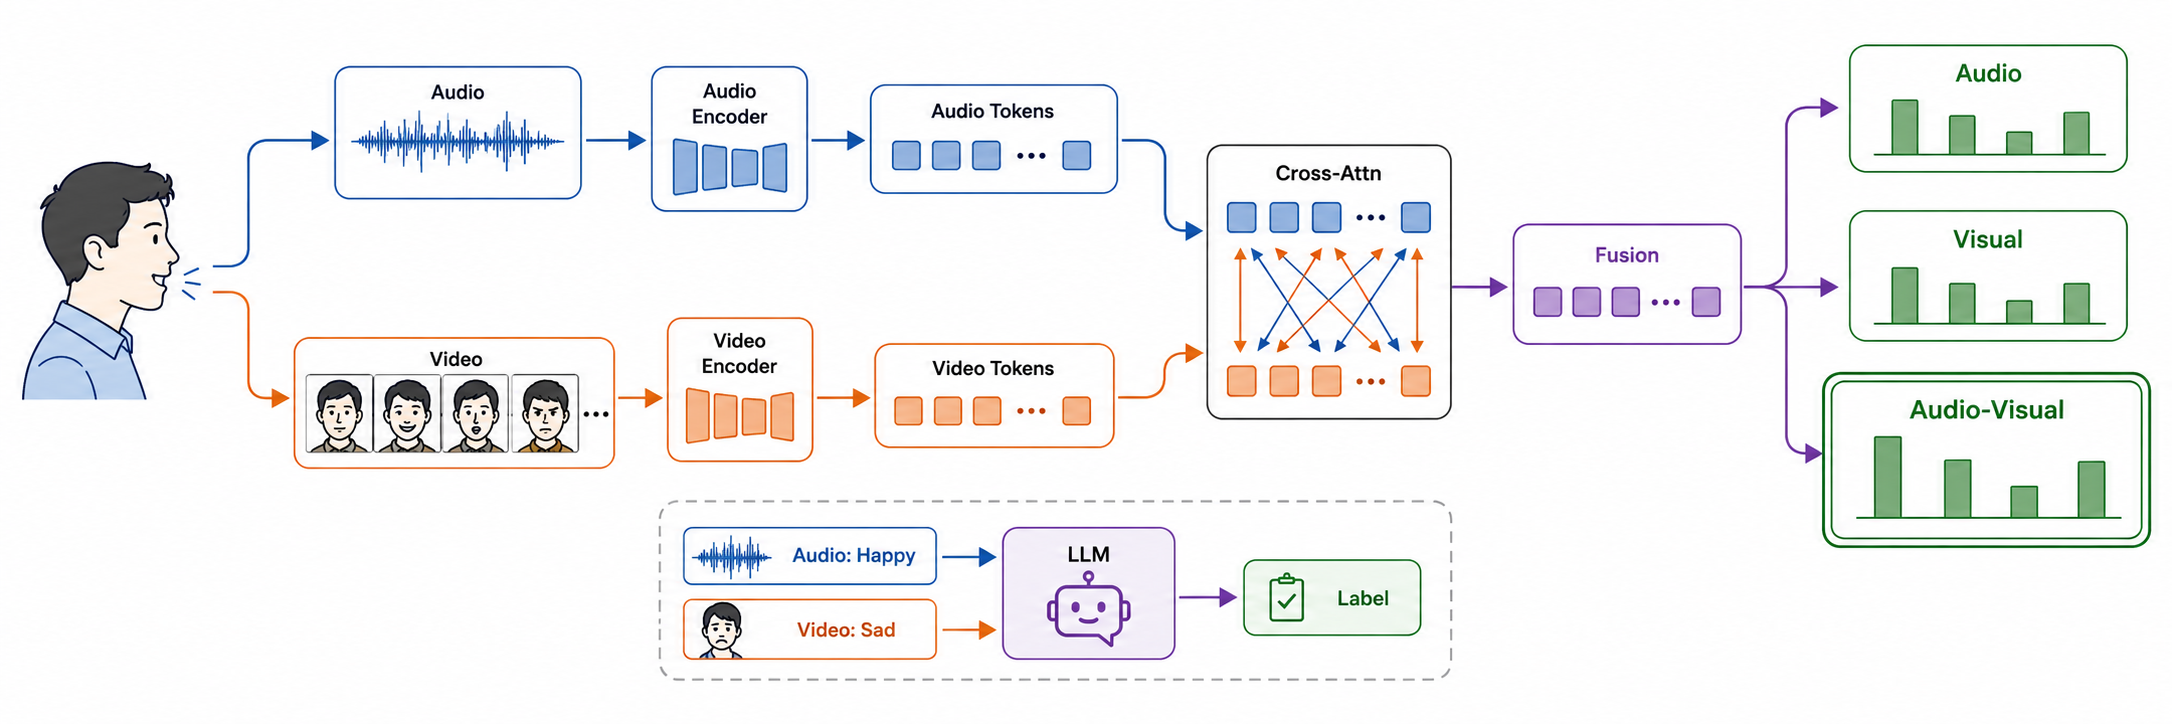
\includegraphics[width=0.92\textwidth]{pineline.png}
  \caption{PAM processing pipeline. WavLM audio tokens and temporally encoded
  EfficientNet face tokens interact through bidirectional cross-attention.
  Audio, video, and fused heads predict six emotions. The dashed projector and
  Qwen path reconciles these predictions when the unimodal branches disagree.}
  \label{fig:arch}
\end{figure*}

\subsection{Audio and Video Encoders}

Let the waveform input be
$\mathbf{x}^{a}\in\mathbb{R}^{B\times T}$. WavLM-base-plus produces a sequence
of 768-dimensional speech states. A linear layer, layer normalization, and
dropout project these states to
$\mathbf{A}\in\mathbb{R}^{B\times T_a\times d}$ with $d=256$. Padding masks
are propagated through WavLM and used by every subsequent attention and
pooling operation.

For video, 16 RGB frames are sampled from each clip. Each detected face is
resized to $224\times224$ and encoded independently by EfficientNet-B0,
producing a 1280-dimensional frame representation. A linear projection maps
the frame features to $d=256$. A two-layer Transformer encoder with four
attention heads and GELU feed-forward blocks models facial motion across the
sampled sequence:
\begin{equation}
  \mathbf{V} =
  \operatorname{Transformer}_{2}
  \left(\operatorname{Proj}_{v}(\operatorname{EffNet}(\mathbf{x}^{v}))\right).
\end{equation}
The selected model freezes the lower pretrained blocks and fine-tunes only the
final two WavLM Transformer layers and final two EfficientNet feature stages.
Projection, temporal, fusion, normalization, and classification modules remain
fully trainable. The model contains 101.16M parameters, of which 18.08M are
updated.

\subsection{Bidirectional Cross-Attention and Gating}

Audio and video sequences have different lengths and are not assumed to be
index-aligned. Two multi-head attention modules exchange context:
\begin{align}
  \mathbf{A}' &=
  \operatorname{LN}\left(
  \mathbf{A}+
  \operatorname{MHA}(\mathbf{A},\mathbf{V},\mathbf{V})
  \right), \\
  \mathbf{V}' &=
  \operatorname{LN}\left(
  \mathbf{V}+
  \operatorname{MHA}(\mathbf{V},\mathbf{A},\mathbf{A})
  \right).
\end{align}
The first expression asks which facial states support each speech state; the
second asks which speech states support each facial state. Invalid positions
are masked before attention. Masked temporal means then produce
$\bar{\mathbf{a}}$ and $\bar{\mathbf{v}}$.

A feature-wise gate determines the mixture:
\begin{equation}
  \mathbf{g} =
  \sigma\!\left(\mathbf{W}_{g}
  [\bar{\mathbf{a}};\bar{\mathbf{v}}]+\mathbf{b}_{g}\right),
  \quad
  \mathbf{e} =
  \operatorname{LN}\left(
  \mathbf{g}\odot\bar{\mathbf{a}}+
  (1-\mathbf{g})\odot\bar{\mathbf{v}}\right).
\end{equation}
Three dropout-linear heads map $\bar{\mathbf{a}}$,
$\bar{\mathbf{v}}$, and $\mathbf{e}$ to six-class audio, video, and fusion
logits. The fusion head is the benchmark output.

\subsection{Joint Hard and Perceptual Objective}
\label{ssec:loss}

The selected model combines label-smoothed categorical supervision with
modality-matched perceptual distributions. Its hard-label component is
\begin{equation}
  \mathcal{L}_{hard} =
  0.75\mathcal{L}^{av}_{CE}
  +0.2\mathcal{L}^{a}_{CE}
  +0.05\mathcal{L}^{v}_{CE},
  \label{eq:hardloss}
\end{equation}
where cross-entropy uses label smoothing 0.05. The larger fusion weight
prioritizes the deployed output while retaining branch-specific supervision.

For the perceptual extension, vote counts $n_c^{(m)}$ under condition $m$ are
converted to Laplace-smoothed distributions:
\begin{equation}
  \tilde{p}^{(m)}_c =
  \frac{n^{(m)}_c+\alpha}
       {\sum_{j=1}^{6}n^{(m)}_j+6\alpha},
  \qquad \alpha=1.
\end{equation}
If a clip-condition pair has no votes, its intended hard emotion is used as an
explicit fallback. The final objective is
\begin{equation}
\begin{aligned}
  \mathcal{L}={}&\mathcal{L}_{hard}
  +0.15D_{KL}(\tilde p_{av}\|p_{av})\\
  &+0.05D_{KL}(\tilde p_{voice}\|p_a)
  +0.02D_{KL}(\tilde p_{face}\|p_v).
\end{aligned}
\end{equation}
These terms preserve a sharp categorical anchor while transferring human
perceptual disagreement to the matching branch.

\subsection{Language-Model Reconciler and Safety Routing}

The dashed branch in Fig.~\ref{fig:arch} is designed for interpretable
reconciliation rather than replacing the classifier. A projector concatenates
the 256-dimensional fusion embedding, the two six-class unimodal probability
vectors, and one audio--video disagreement scalar. Two linear layers reshape
the resulting 269-dimensional vector into four prefix embeddings. These are
prepended to the prompt embeddings of
Qwen2.5-0.5B-Instruct~\cite{qwen2025}. The base language model is frozen and
rank-16 LoRA adapters~\cite{hu2022lora} are attached to its query, key, value,
and output projections.

The textual prompt names the six-class audio, video, and fusion probability
vectors together with the disagreement value. During adaptation, common
prompt tokens are masked and supervision is applied only to the target emotion
tag. At inference, each of the six valid tags is scored by conditional
negative log-likelihood, preventing unconstrained generations from changing
the label space. The four 896-dimensional prefix tokens and 2.16M LoRA
parameters are trainable; the PAM encoders and Qwen base weights remain
frozen.

Because a reconciler can degrade reliable classifier decisions, PAM-VLM uses
a validation-selected safety rule. Qwen is consulted only when audio--video
disagreement is at least 0.324 and PAM confidence is at most 0.665; otherwise
the fusion prediction is retained. The rule is selected on Mini-CREMA
validation data and transferred unchanged to RAVDESS.

\section{Experimental Setup}
\label{sec:setup}

This section states the complete setup used to produce the reported values.
The distinction between training, model selection, and final evaluation is
maintained throughout.

\subsection{Dataset and Clip-Level Split}

The input corpus is the complete CREMA-D release: 7,442 clips, 91 actors, six
emotion classes, and paired audio/video media. The primary split is generated
once with seed 42 and stratification by hard emotion. The five non-neutral
classes each contain 1,271 clips; neutral contains 1,087. Stratification
produces 5,954 training, 744 validation, and 744 test clips.

No clip ID is shared across partitions. All 91 actors occur in all three
partitions by design, so identity overlap is not accidental leakage but a
declared property of the protocol. The split answers: ``How accurately can the
model classify unseen clips drawn from the same actor population?'' It does
not answer: ``How accurately does the model generalize to a new actor?''

The split is created once before training and then held fixed for every model.
Class identities and clip membership are unchanged across the audio-only,
video-only, and fusion experiments. Test labels are never used for tuning or
checkpoint selection.

\subsection{Media Preprocessing}

Audio is decoded as a mono waveform and resampled to 16~kHz. Variable-length
waveforms are padded within each mini-batch, and a Boolean mask prevents padded
samples from contributing to WavLM attention or temporal pooling. No
spectrogram is computed because WavLM consumes waveform samples directly.

Video is decoded with OpenCV. During training, 16 frame indices are sampled
without replacement when enough frames are available; validation uses 16
deterministic linearly spaced indices. An offline Haar cascade detects a face
in each frame. The detected square is expanded by a 15\% margin and resized to
$224\times224$. A center-square crop is used when detection fails. RGB values
are converted to floating point in $[0,1]$.

Augmentation is restricted to the training partition and applied with
probability 0.8 independently for each modality pipeline. Audio augmentation
uses a circular shift of at most 10\% of waveform length, gain in
$[0.9,1.1]$, Gaussian noise with standard deviation 0.005 times signal RMS,
and polarity inversion with probability 0.5. Video augmentation applies one
clip-consistent horizontal flip with probability 0.5 and brightness/contrast
jitter of at most 0.2. Validation and test media receive no random
augmentation.

\subsection{Model and Optimization Settings}

Table~\ref{tab:setup} consolidates the model and training setup. All reported
models use the same split, preprocessing, augmentation policy, and seed. The
audio-only, video-only, and frozen-fusion runs provide controlled baselines.
The selected high-accuracy model then changes the fine-tuning and regularization
settings listed below; its contribution is therefore measured relative to the
frozen-fusion baseline as well as the unimodal models.

\begin{table}[t]
\centering
\caption{Implementation and training setup for the reported primary runs.}
\label{tab:setup}
\footnotesize
\setlength{\tabcolsep}{4pt}
\renewcommand{\arraystretch}{1.04}
\begin{tabular}{@{}p{0.25\columnwidth}p{0.69\columnwidth}@{}}
\toprule
\textbf{Component} & \textbf{Configuration} \\
\midrule
Audio input
  & 16-kHz waveform; masked variable-length batches \\
Video input
  & 16 RGB face frames, $224\times224$; 15\% crop margin \\
Audio encoder
  & WavLM-base-plus; final two layers trainable; 768-D to 256-D \\
Video encoder
  & EfficientNet-B0; final two stages trainable; 1280-D to 256-D \\
Fusion
  & Two 4-head cross-attention directions; audio gate bias 1.5 \\
Regularization
  & Fusion dropout 0.15; head dropout 0.25; modality dropout 0.2 \\
Objective
  & Weighted CE with smoothing 0.05 and modality-matched KL \\
Optimization
  & AdamW; task LR $2\times10^{-4}$; backbone LR $10^{-5}$; WD 0.01 \\
Training budget
  & At most 40 epochs; batch 4; accumulation 8; patience 8 \\
Model selection
  & Maximum validation Macro-F1; epoch 24 selected \\
\bottomrule
\end{tabular}
\end{table}

AdamW uses $2\times10^{-4}$ for task and fusion layers and $10^{-5}$ for the
unfrozen backbone blocks. Cosine annealing reduces the task learning rate to
$10^{-6}$. A physical batch size of 4 with eight accumulation steps gives an
effective batch size of 32. Mixed precision is enabled and the gradient norm
is clipped at 1.0. The best validation Macro-F1 occurs at zero-indexed epoch
24. Training stops after epoch 32 when eight subsequent epochs fail to improve
the selection metric.

\subsection{Reconciler Adaptation and Transfer Protocol}

The language branch is adapted on a balanced Mini-CREMA subset containing 780
training clips (130 per class) and 120 validation clips (20 per class). This
subset is used only to establish whether the projector, LoRA adapters, and
safety routing improve a fixed PAM classifier; it contains no samples from the
primary 744-clip CREMA-D test partition. PAM features and probability vectors
are cached, while Qwen LoRA parameters and the projector are optimized with
learning rates of $2\times10^{-5}$ and $2\times10^{-4}$, respectively. The
physical batch size is 4 with four accumulation steps. Epoch 1 is selected by
validation Macro-F1.

Cross-corpus transfer uses RAVDESS~\cite{livingstone2018ravdess}, restricted to
the six labels shared with CREMA-D. The complete prepared evaluation set
contains 1,056 clips from 24 actors. No RAVDESS labels are used for adaptation
or threshold selection. The frozen PAM, Qwen reconciler, and safety router are
evaluated once on all 1,056 clips. The same Mini-CREMA-selected routing
thresholds are also evaluated on the untouched 744-clip CREMA-D test set.

\subsection{Evaluation Metrics and Decision Rule}

For class $c$, precision and recall are
\begin{equation}
 P_c=\frac{TP_c}{TP_c+FP_c}, \qquad
 R_c=\frac{TP_c}{TP_c+FN_c}.
\end{equation}
Class F1 is $F1_c=2P_cR_c/(P_c+R_c)$. With $C=6$, the two primary metrics are
\begin{equation}
 \operatorname{MacroF1}=\frac{1}{C}\sum_{c=1}^{C}F1_c,
 \qquad
 \operatorname{UAR}=\frac{1}{C}\sum_{c=1}^{C}R_c.
\end{equation}
Accuracy is the number of correct predictions divided by the number of
samples. Macro-F1 is the checkpoint-selection metric because it weights all
classes equally and penalizes both low precision and low recall. UAR isolates
recall balance, while accuracy preserves comparability with papers that report
only recognition rate. Calibration is summarized with 15-bin expected
calibration error (ECE):
\begin{equation}
  \operatorname{ECE}=\sum_{b=1}^{15}\frac{|B_b|}{N}
  \left|\operatorname{acc}(B_b)-\operatorname{conf}(B_b)\right|.
\end{equation}

The development decision rule is fixed before testing: compare candidate
models on validation Macro-F1, freeze the selected architecture and
hyperparameters, and evaluate the 744-clip test partition once. This procedure
has now been completed; the primary numbers below are held-out test results.

\section{Results}
\label{sec:results}

\subsection{Training and Model Selection}

Figure~\ref{fig:training} summarizes optimization of the selected model. The
training loss decreases throughout the run, while validation loss falls
rapidly and then stabilizes near 0.72. Validation Macro-F1 increases from
approximately 0.73 to 0.906. At the selected epoch 24, train and validation
Macro-F1 are 0.987 and 0.906, respectively, and train/validation losses are
0.570/0.725. The gap indicates residual overfitting, but validation performance
does not collapse. Early stopping after epoch 32 prevents further optimization
after eight non-improving epochs.

\begin{figure*}[t]
  \centering
  \begin{minipage}[t]{0.49\textwidth}
    \centering
    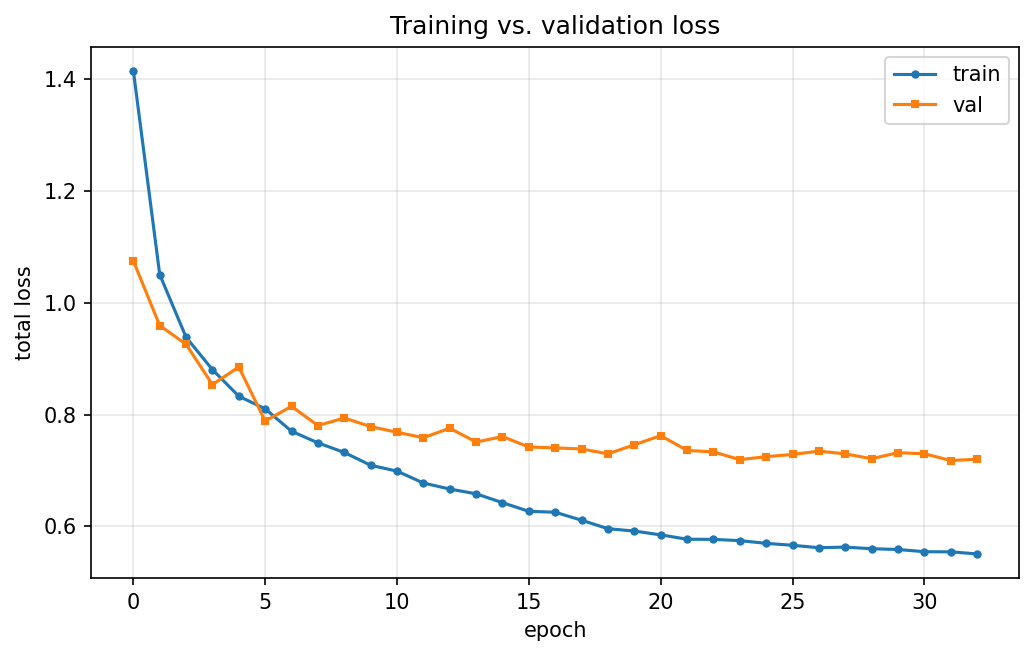
\includegraphics[width=\linewidth]{pam_highacc_loss_curves.png}\\[-2pt]
    \small (a) Training and validation objective.
  \end{minipage}\hfill
  \begin{minipage}[t]{0.49\textwidth}
    \centering
    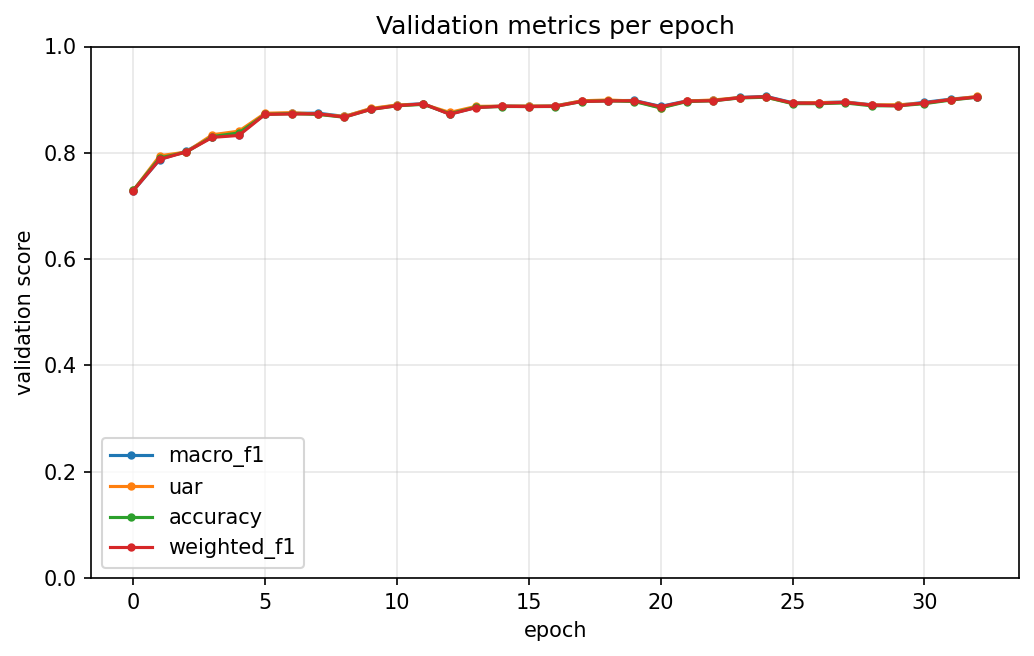
\includegraphics[width=\linewidth]{pam_highacc_metric_curves.png}\\[-2pt]
    \small (b) Validation classification metrics.
  \end{minipage}
  \caption{Learning curves for the selected high-accuracy model. The best
  validation Macro-F1 occurs at epoch 24; training terminates after epoch 32
  under patience 8.}
  \label{fig:training}
\end{figure*}

\subsection{Overall Validation and Test Results}

\begin{table*}[t]
\centering
\caption{Validation and held-out test results under the shared clip-level
80/10/10 split. ECE uses 15 confidence bins. Bold denotes the best test value.}
\label{tab:results}
\small
\setlength{\tabcolsep}{8pt}
\begin{tabular}{lccccc}
\toprule
\textbf{Model} & \textbf{Val. Macro-F1} & \textbf{Test Macro-F1}
& \textbf{Test UAR} & \textbf{Test Accuracy} & \textbf{Test ECE} \\
\midrule
Audio-only                   & 0.738 & 0.720 & 0.720 & 0.719 & 0.057 \\
Video-only                   & 0.736 & 0.702 & 0.697 & 0.696 & 0.062 \\
Frozen fusion, hard labels   & 0.832 & 0.849 & 0.845 & 0.847 & \textbf{0.038} \\
\textbf{PAM high-accuracy}   & \textbf{0.906} & \textbf{0.888}
  & \textbf{0.886} & \textbf{0.887} & 0.090 \\
\bottomrule
\end{tabular}
\end{table*}

The final test results in Table~\ref{tab:results} confirm the validation-based
selection. PAM reaches 0.888 Macro-F1, 0.886 UAR, and 0.887 accuracy. Relative
to frozen hard-label fusion, selective fine-tuning and the joint objective add
3.93 Macro-F1, 4.02 UAR, and 4.03 accuracy points. The gain over audio-only is
16.78 Macro-F1 points, and the gain over video-only is 18.59 points. Validation
Macro-F1 exceeds test Macro-F1 by 1.80 points, a moderate selection gap rather
than a reversal of model ranking.

The improvement has a calibration cost. ECE increases from 0.038 for frozen
fusion to 0.090 for the high-accuracy model, even though its classification
metrics are substantially better. Temperature scaling on a separate
calibration subset is therefore a suitable deployment step, but it must not be
fit on the held-out test set.

\subsection{Language Reconciliation and Cross-Corpus Transfer}

\begin{table*}[t]
\centering
\caption{PAM-VLM reconciliation results. Mini-CREMA is validation data used
for checkpoint and routing selection; CREMA-D test and RAVDESS zero-shot are
full evaluations with frozen thresholds.}
\label{tab:vlm}
\small
\setlength{\tabcolsep}{8pt}
\begin{tabular}{llrrrr}
\toprule
\textbf{Evaluation} & \textbf{Decision system} & \textbf{Samples}
& \textbf{Macro-F1} & \textbf{UAR} & \textbf{Accuracy} \\
\midrule
\multirow{3}{*}{Mini-CREMA validation}
  & PAM & 120 & 0.8750 & 0.8750 & 0.8750 \\
  & Qwen reconciler & 120 & 0.8919 & 0.8917 & 0.8917 \\
  & PAM+VLM routing & 120 & \textbf{0.8924} & \textbf{0.8917} & \textbf{0.8917} \\
\addlinespace[2pt]
\multirow{3}{*}{CREMA-D held-out test}
  & PAM cache baseline & 744 & \textbf{0.8870} & \textbf{0.8846} & \textbf{0.8858} \\
  & Qwen reconciler & 744 & 0.8750 & 0.8727 & 0.8737 \\
  & PAM+VLM routing & 744 & 0.8817 & 0.8791 & 0.8804 \\
\addlinespace[2pt]
\multirow{3}{*}{RAVDESS zero-shot}
  & PAM & 1,056 & \textbf{0.5618} & \textbf{0.5573} & \textbf{0.5634} \\
  & Qwen reconciler & 1,056 & 0.5004 & 0.5226 & 0.5312 \\
  & PAM+VLM routing & 1,056 & 0.5071 & 0.5278 & 0.5369 \\
\bottomrule
\end{tabular}
\end{table*}

On Mini-CREMA, direct Qwen reconciliation improves Macro-F1 by 1.69 points
over PAM, and safety routing reaches 0.8924. This is validation evidence
rather than an independent test result because the checkpoint and thresholds
are selected on the same 120 samples.

The held-out evaluations reverse that ordering. On CREMA-D test, direct Qwen
reduces Macro-F1 by 1.20 points and routing reduces it by 0.53 points relative
to the cached PAM baseline while routing 60.6\% of clips. On RAVDESS, PAM
obtains 0.5618 Macro-F1, while Qwen and routing obtain 0.5004 and 0.5071,
respectively. Routing is activated for 35.4\% of RAVDESS clips. The result
shows that Mini-CREMA confidence and disagreement thresholds do not generalize
reliably to held-out or cross-corpus samples.

\begin{table*}[t]
\centering
\caption{Published audio--visual RAVDESS context. Protocols and label sets
differ, so the values are not a common leaderboard.}
\label{tab:ravdess}
\small
\setlength{\tabcolsep}{8pt}
\begin{tabular}{@{}lllc@{}}
\toprule
\textbf{Study} & \textbf{Evaluation protocol} & \textbf{Labels}
& \textbf{Accuracy (\%)} \\
\midrule
MATER~\cite{ghaleb2023mater}
  & Paper-defined audio--visual evaluation & Paper-defined & 76.30 \\
Luna-Jimenez \emph{et al.}~\cite{lunajimenez2021ravdess}
  & Subject-wise five-fold & 8 classes & 80.08 \\
Middya \emph{et al.}~\cite{middya2022fusion}
  & Random 80/10/10 & 8 classes & 86.00 \\
Mocanu \emph{et al.}~\cite{mocanu2023crossmodal}
  & Paper-defined audio--visual evaluation & Paper-defined & 89.25 \\
CAMS~\cite{lei2026cams}
  & Paper-defined audio--visual evaluation & Paper-defined & 89.78 \\
\midrule
PAM zero-shot
  & All 1,056 clips; no RAVDESS adaptation & 6 classes & 56.34 \\
PAM+VLM zero-shot
  & All 1,056 clips; no RAVDESS adaptation & 6 classes & 53.69 \\
\bottomrule
\end{tabular}
\end{table*}

Table~\ref{tab:ravdess} places the zero-shot result near established
audio--visual methods without claiming direct superiority. The published
studies train and test on RAVDESS, whereas PAM receives no RAVDESS
adaptation and uses only the six labels shared with CREMA-D. The substantially
lower score therefore measures cross-corpus transfer rather than
within-RAVDESS supervised recognition.

\subsection{Class-Level Analysis}

\begin{table}[t]
\centering
\caption{Per-class performance of PAM high-accuracy on the 744-clip test set.}
\label{tab:class}
\small
\setlength{\tabcolsep}{5.2pt}
\begin{tabular}{lrrrr}
\toprule
\textbf{Emotion} & \textbf{Precision} & \textbf{Recall} & \textbf{F1} & \textbf{Support} \\
\midrule
Angry   & 0.914 & 0.921 & 0.918 & 127 \\
Disgust & 0.908 & 0.929 & 0.918 & 127 \\
Fear    & 0.844 & 0.811 & 0.827 & 127 \\
Happy   & 0.992 & 0.953 & 0.972 & 127 \\
Neutral & 0.957 & 0.826 & 0.887 & 109 \\
Sad     & 0.750 & 0.874 & 0.807 & 127 \\
\bottomrule
\end{tabular}
\end{table}

Happiness is the most reliable class, with 0.972 F1 and 121/127 correct
predictions. Angry and disgust both reach approximately 0.918 F1. Neutral has
high precision (0.957) but lower recall (0.826), whereas sadness has the lowest
precision (0.750) and 0.874 recall. The close aggregate values for Macro-F1,
UAR, and accuracy indicate that the final score is not produced by one
dominant class.

\begin{figure}[t]
  \centering
  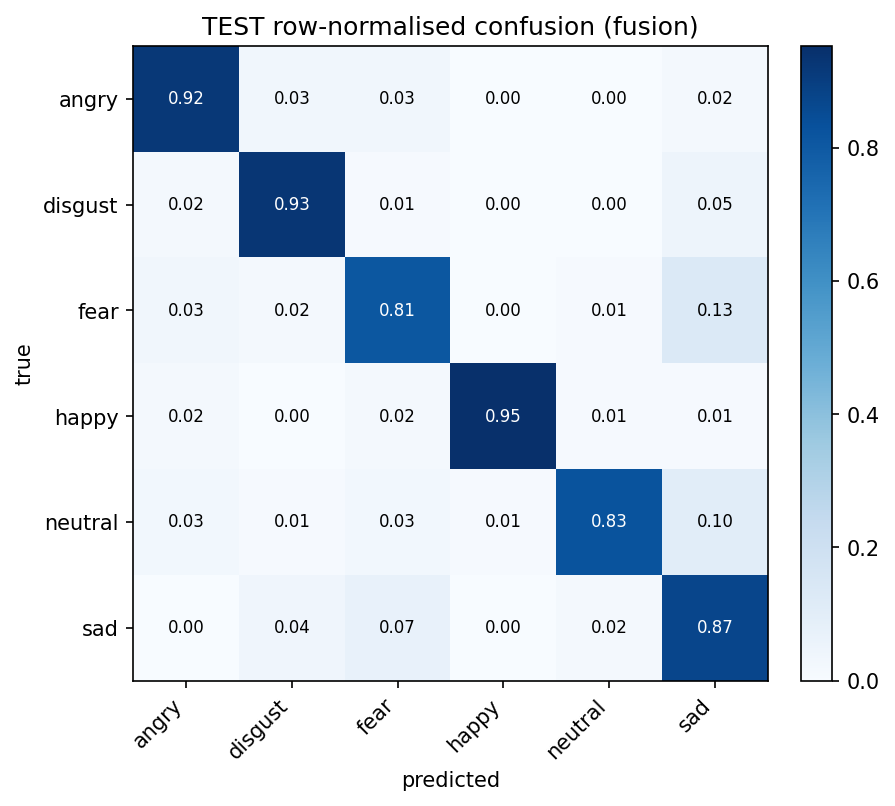
\includegraphics[width=0.92\columnwidth]{pam_highacc_test_confusion_matrix_norm.png}
  \caption{Row-normalized confusion matrix of PAM high-accuracy on the held-out
  test partition. Rows are true classes and columns are predictions.}
  \label{fig:confusion}
\end{figure}

Figure~\ref{fig:confusion} shows that the principal residual error is attraction
toward sadness: 17 fear and 11 neutral clips are predicted as sad. In the
opposite direction, nine sad clips are predicted as fear. This pattern explains
sadness's low precision and fear's lower recall. Class-conditional reliability
modeling should therefore focus on the fear--sad and neutral--sad boundaries.

\subsection{Position Relative to Published Work}

Within the random or clip-level family, PAM's 88.71\% test accuracy is
numerically above OTM's 75.10\%, Wang \emph{et al.}'s 88.29\%, and FMII's
$88.21\pm0.34$\%. PAM's 88.82\%
Macro-F1 is also above the 84.50\% reported by Wang \emph{et al.} These
values define context rather than universal superiority because even the
closest studies differ in split ratios, seed averaging, feature encoders, and
model-selection procedures.

Speaker-independent and cross-validation results in the first block of
Table~\ref{tab:literature} answer a harder identity-generalization question
and are deliberately not ranked against PAM. A strict comparison requires
retraining accessible baselines on the PAM manifest over matched seeds. The
present evidence supports strong clip-level within-corpus recognition, not a
protocol-independent state-of-the-art claim.

\section{Discussion and Future Work}
\label{sec:improvements}

\subsection{Effect of Selective Fine-Tuning}

The 3.93-point test Macro-F1 gain over frozen fusion shows that generic
pretrained representations remain improvable for acted emotion recognition.
Restricting updates to upper backbone blocks adapts high-level acoustic and
facial cues without optimizing all 101.16M parameters. Modality dropout and
the audio-biased gate further discourage dependence on one stream, while the
KL terms connect each branch to the matching perceptual condition.

The experiment changes several components together, so the gain cannot yet be
attributed to one mechanism. A factorial ablation should add selective
fine-tuning, modality dropout, gate bias, label smoothing, and perceptual KL
sequentially under the same split. This is more informative than treating the
combined high-accuracy configuration as evidence that every component helps.

\subsection{Error-Driven Improvements}

The confusion pattern suggests tracked, aligned face crops to reduce temporal
jitter and class-conditional reliability gates that can favor speech for one
emotion and facial motion for another. A confusion-aware loss is justified
only if repeated seeds confirm the sadness false-positive pattern.

Improvements should be staged: selective fine-tuning, modality dropout,
perceptual KL supervision, then reliability gating. Each stage uses the same
split and reports its incremental Macro-F1. Three to five seeds should
estimate variance before a final ensemble is considered.

\subsection{Role of the Language Model}

The Mini-CREMA result shows that language-model reconciliation can fit a small
subset of uncertain in-domain decisions. The two full evaluations show that
this gain does not survive held-out testing or cross-corpus transfer. Routing
more samples is harmful when confidence and disagreement distributions shift.
Qwen is not a native audio--visual foundation model in this system. It receives
compact PAM evidence through learned prefix tokens and returns one of six
constrained labels.

Required ablations are Qwen without LoRA, LoRA without routing, alternative
calibration scores, and routing learned on a larger held-out development set.
Any new router must be selected without test labels. Generated rationales
remain secondary to label accuracy.

\section{Limitations and Threats to Validity}
\label{sec:limitations}

The main limitation is deliberate actor overlap. Recurring voice, face, or
sentence cues may make the task easier than unseen-speaker evaluation. The
result comes from one corpus and one split seed; a different partition may
change it. Although the test partition was evaluated only after model
selection, repeated seeds are still required to estimate variance.

CREMA-D contains acted English recorded under controlled conditions.
Performance may not transfer to spontaneous emotion, other languages, noisy
media, or asynchronous streams. Haar detection is reproducible but less robust
than modern alignment, and missing-stream robustness remains unmeasured.

External validity is further limited by protocol mismatch across published
work. Some papers average multiple speaker-independent folds, while others use
one random clip split. Accuracy, UAR, and Macro-F1 are not interchangeable.
For these reasons, Table~\ref{tab:literature} is descriptive and the report
does not claim a universal ranking.

The current language-model evidence has two additional boundaries.
Mini-CREMA reports the same validation set used for checkpoint and routing
selection, so it is not a held-out performance claim. The RAVDESS evaluation
covers the complete prepared set, but its six-class mapping and zero-shot
CREMA-D training differ from the supervised eight-class protocols in prior
work. Neither language-model result replaces the primary PAM test score.

\section{Ethical Considerations}
\label{sec:ethics}

Emotion labels are perceptual judgments, not direct measurements of internal
state. Predictions reflect acting, annotation, demographic, and recording
biases. The system must not be the sole basis for high-stakes decisions.
Deployment requires subgroup evaluation, consent, privacy protection, and a
way to contest inferences. Generated rationales are not factual explanations
of a person's mental state.

\section{Conclusion}
\label{sec:conclusion}

PAM-VLM combines pretrained audio and visual encoders with temporal modeling,
bidirectional cross-attention, and gated pooling for six-class CREMA-D emotion
recognition. Under a deterministic, emotion-stratified 80/10/10 clip-level
split, the selected high-accuracy model reaches 90.61\% validation Macro-F1.
On the held-out test partition it obtains 88.82\% Macro-F1, 88.56\% UAR, and 88.71\%
accuracy. This improves test Macro-F1 by 3.93 points over frozen hard-label
fusion and by more than 16 points over both unimodal models. The setup,
learning curves, class-level errors, and selection rule are reported so that
the experiment can be reproduced and interpreted correctly.

On Mini-CREMA validation, disagreement-aware reconciliation raises Macro-F1
from 87.50\% to 89.24\%. This gain does not hold on the complete evaluations:
routing reduces CREMA-D test Macro-F1 from 88.70\% to 88.17\% and RAVDESS
zero-shot Macro-F1 from 56.18\% to 50.71\%. The negative result identifies
validation overfitting and unresolved cross-corpus shift in the reconciler.

The primary result demonstrates strong within-corpus clip recognition, not
generalization to unseen actors. Multi-seed confirmation, component-wise
ablation, larger routing-development data, cross-corpus calibration, and
stable face tracking are the most direct next steps.

\IEEEtriggeratref{7}
\bibliographystyle{IEEEtran}
\bibliography{refs}

\end{document}
